%!TEX root = thesis.tex
\chapter{Tensor Network Theory} 
\label{chap2}
In this chapter, we will introduce the foundations of tensor network \cite{jordan_studies_2011,Orus2014117,bauer_tensor_2011}, which is a new language for condense matter physics, and explain how to map the quantum many-body states into the tensor network. 
%This section begins from a fundamental question: How to draw a tensor network diagram? In tensor network theory , we are used to represent tensors as the notations, shown in Fig.~\ref{fig211}, because \textit{tensor diagrams} can fully describe the quantum states of any geometric lattice systems explicitly. Furthermore, base on its clear representation, the implementation of tensor network algorithms become simply. 

\section{Representation of tensors in tensor Networks}
\label{notations}

Mathematically, a tensor is considered as a multi-dimensional array of scalars. We can represent a tensor graphically as a circle with bonds for open indices. Each bond represents an \textit{index} of the array, and the number of bonds corresponds to the rank of the tensor, see Fig.~\ref{fig211}. To explain more clearly, if there is a tensor $T_{\alpha \beta \gamma}$ shown as in Fig.~\ref{fig211}(iv) and the dimensions of the each bond $\alpha, \beta$ and $\gamma$ are $\chi_{\alpha},\chi_{\alpha}$ and $\chi_{\gamma}$, $T_{\alpha \beta \gamma}$ contains $\chi_{\alpha}\chi_{\beta}\chi_{\gamma}$ coefficients.

%\begin{align}
%	D_{total} = \begin{cases}
%		1 & \text{, if $N = 0$} \\
%		\chi_{1}\chi_{2}\chi_{3} \dots \chi_{N} & \text{, if $N \neq 0$}
%	\end{cases}
%\end{align}

\begin{figure}[ht]
	\centering
	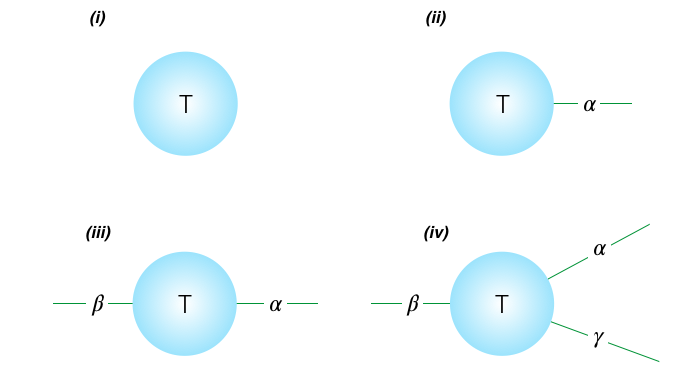
\includegraphics[width=0.75\textwidth]{figures/fig211.png}
	\caption[The reprecentation of commen tensors.]{(i) A tensor without bonds is a scalar $T$, (ii) A tensor with one bond is a vector $T_{\alpha}$, (iii) A tensor with two bonds is a Matrix $T_{\alpha \beta}$, (iv) A tensor with three bonds is a rank-3 tensor $T_{\alpha \beta \gamma}$.}
	\label{fig211}
\end{figure}

\section{Tensor operations and tensor network diagrams} % (fold)
\label{operation}

Since computers can perform the calculation efficiently of matrices, to implement calculations of tensor networks on computers, we need to perform operations on tensors to make them into matrices, such as permutation and reshape. To explain more explicitly, we define a representation at first,


\begin{enumerate}
	\item $T_{[\alpha \beta], \gamma}$: The bonds $\alpha$ and $\beta$ of a tensor $T$ are grouped. It can be recognized as a matrix, which rows and columns are $\chi_{\alpha}\chi_{\beta}$ and $\chi_{\gamma}$. We will discuss more more details in Sec.~\ref{reshape}
\end{enumerate}

\subsection{Permutation}

The permutation operation is to re-order the arrangement of the coefficients in a tensor according to some specified ordering of the bonds. As shown in Fig.~\ref{fig224}, we permute the tensor $A$ to $\hat{A}$, where the arrangement of the coefficients of the tensor $\hat{A}$ is determined by the assignment $\hat{A}_{\alpha \gamma \beta} = A_{\alpha \beta \gamma}$.

\begin{figure}[H]
	\centering
	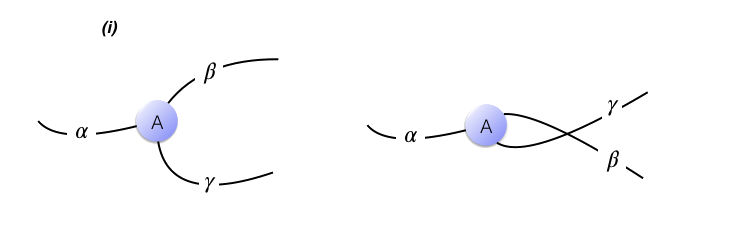
\includegraphics[width=0.75\textwidth]{figures/fig224.png}
	\caption[The permutation of a tensor.]{ Permute tensor $A_{\alpha \beta \gamma}$ to $\hat{A}_{\alpha \gamma \beta}$ }
	\label{fig224}
\end{figure}

\subsection{Reshape}
\label{reshape}
The reshape operation is to combined more than two bonds of a tensor into a single bond. Although the rank of the tensor is reduced, the arrangement of coefficients is unchanged. The dimension of the new bond is equal to the product of the dimensions of the bonds contained in it. As shown in Fig.~\ref{figreshape}, we joint the bonds $\alpha$ and $\beta$ into a new bond $\delta$. Assume that the dimension of the bonds $\alpha$ and $\beta$ are $\chi_{\alpha}$ and $\chi_{\beta}$. The dimension of the bond $\delta$ is equal to $\chi_{\alpha}\chi_{\beta}$. In this thesis, we write down this operation as\begin{align}
	T_{\alpha, \delta} = T_{\alpha, \beta \gamma}
\end{align}

\begin{figure}[H]
	\centering
	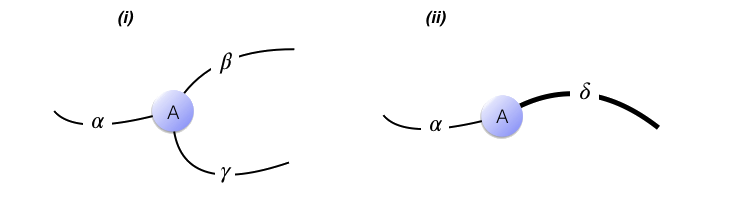
\includegraphics[width=0.75\textwidth]{figures/figreshape.png}
	\caption[The permutation of a tensor.]{ Permute tensor $A_{\alpha \beta \gamma}$ to $\hat{A}_{\alpha \gamma \beta}$ }
	\label{figreshape}
\end{figure} 

%\begin{align}
%	A_{\alpha \beta \gamma} \rightarrow \hat{A}_{\alpha \gamma \beta}
%\end{align}

%Nevertheless, the arrangements of tensor $A_{\alpha \beta \gamma}$ is modified to $\hat{A}_{\alpha \gamma \beta}$. The components of them are exact equivalence. 
%
%\begin{figure}[ht]
%	\centering
%	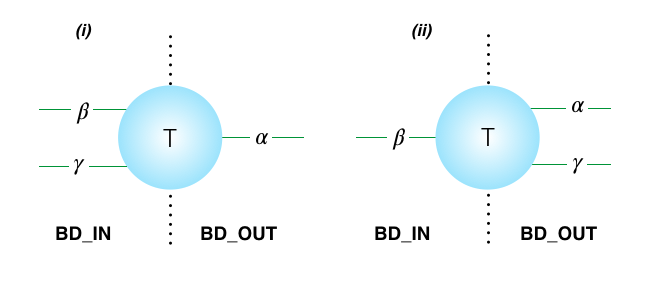
\includegraphics[width=0.80\textwidth]{figures/fig221.png}
%	\caption[Representaion of unfold tensors.]{(i) Unfold a tensor to a matrix $T_{\chi_{\beta}\chi_{\gamma},\chi_{\alpha}}$, (ii) Unfold a tensor to a matrix $T_{\chi_{\beta},\chi_{\alpha}\chi_{\gamma}}$.}
%	\label{fig221}
%\end{figure}

%In order to explain more clearly, we separate the tensor to two part, incoming (BD\_IN) and outgoing (BD\_OUT) which are also designed for distinguishing different types of \textit{uni10::Bond} in \textit{Uni10 Library} \cite{}, to show what the meaning of reshape is in the linear algebra. The total dimensions of the bonds in the part BD\_IN and BD\_OUT corresponds to the number of rows and columns of a matrix. For instance, if the indices of $T_{\alpha \beta \gamma}$ ordered like Fig.~\ref{fig221}(i), $T_{\alpha \beta \gamma}$ is equivalent to a matrix $M_{\chi_{\beta}\chi_{\gamma},\chi_{\alpha}}$, where $\chi_{\alpha}$, $\chi_{\beta}$ and $\chi_{\gamma}$ are the dimensions of the bonds, $\alpha$, $\beta$ and $\gamma$. Similarity, The tensor shown as Fig.~\ref{fig221}(ii) can be recognized as a matrix $M_{\chi_{\beta},\chi_{\alpha}\chi_{\gamma}}$.

\subsection{Tensor contraction}

Tensor contraction is defined as the sum of all products of the shared indices of tensors. For instance, the tensor diagram of contracting two rank-2 tensors $A_{\alpha \beta}$ and $B_{\beta \gamma}$ is shown as Fig.~\ref{fig222}(i) which can be written as
\begin{align}
	C_{\alpha \gamma}=\sum\limits_{\beta = 1}^{\chi_{\beta}}{A_{\alpha \beta}B_{\beta \gamma}},
\end{align}
where $\chi_{\beta}$ is the dimension of the bond $\beta$, and it can be regarded as the inner-product of two matrices $A$ and $B$. Now we extend to a more complicated example [Fig.~\ref{fig222}(ii)], the tensor diagram corresponds to 
\begin{align}
	D_{\alpha \gamma \sigma \epsilon}=\sum_{\beta \rho \delta}{A_{\rho \beta}B_{\beta \sigma \epsilon \delta}C_{\gamma \delta \rho \alpha}}.
\end{align}
In this case, we want to contract bonds $\rho,\beta$ and $\delta$ whose dimensions are $\chi_{\rho}, \chi_{\beta}$ and $\chi_{\delta}$, respectively. Hence, we can complete the contraction processes by the following steps,

\begin{figure}[H]
	\centering
	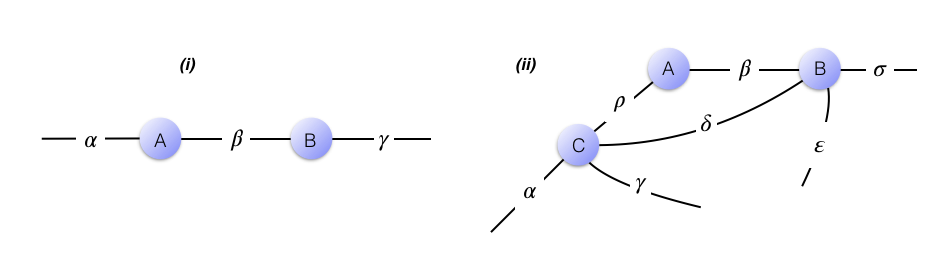
\includegraphics[width=0.75\textwidth]{figures/fig222.png}
	\caption[The examples of tensor diagrams.]{(i) Contract rank-2 tensors $A_{\alpha \beta}$ and $B_{\beta \gamma} $ (ii) Contract a rank-2 tensor $A_{\rho \beta}$, and two rank-4 tensors $B_{\sigma \varepsilon \delta}$ and $C_{\delta \rho \alpha}$}
	\label{fig222}
\end{figure}

\begin{figure}[ht]
	\centering
	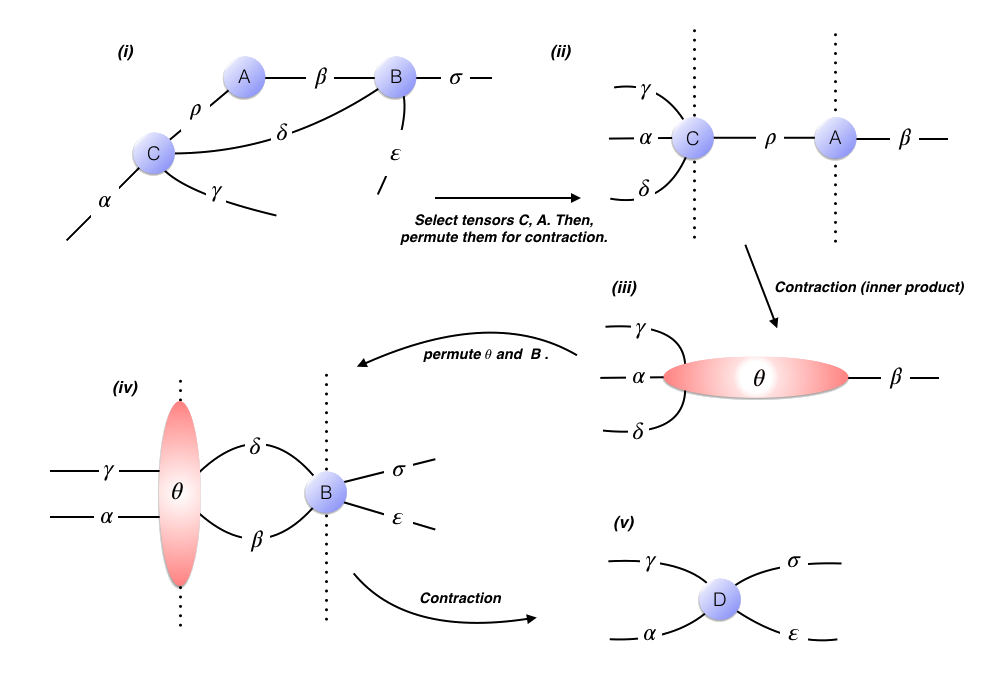
\includegraphics[width=0.75\textwidth]{figures/fig223.png}
	\caption[The contraction procedures of the network shown in Fig\ref{fig222}(ii)]{ The contraction procedures of the network shown in Fig\ref{fig222}}
	\label{fig223}
\end{figure}

\begin{enumerate}

	\item Select a pair of tensors arbitrarily: In the example, we choose the tensor $A_{\rho \beta}$ and $C_{\gamma \alpha \delta \rho}$ at first. 
	\item Permute the tensors to specific shapes and perform the inner-product: As shown in Fig.~\ref{fig223}(ii)-(iii) Permute $A_{\rho \beta}$ and $C_{\gamma \alpha \delta \delta}$ to the specific shape $A_{\rho, \beta}$ and $C_{[\gamma \alpha \delta], \rho}$, which can be regarded as inner product of two matrices $A$ and $C$, 
		\begin{align}
			\theta_{\gamma \alpha \delta \beta} = \sum_{\rho = 1}^{\chi_{\rho}}{C_{[\gamma \alpha \delta], \rho} A_{\rho, \beta}}
		\end{align}
	\item Repeat the step (1) and (2) until all tensors are contracted: See Fig.~\ref{fig223}(iii)-(iv), repeat the steps again to contract the remained tensors $\theta_{\gamma \alpha \delta \beta}$ and $B_{\beta \sigma \delta \varepsilon}$.
\end{enumerate}
%Actually, the choice in step (1) is restricted in some algorithms, such as corner transfer matrix \cite{PhysRevB.85.205117} and fast full update \cite{PhysRevB.92.035142}, because the order of the contraction network is strongly correlated to the efficiency. For example, if the dimensions of the bonds of the tensors, $A_{\rho \beta}$, $B_{\beta \sigma \epsilon \delta}$ and $C_{\gamma \delta \rho \alpha}$ in Fig.~\ref{fig223}(i), are $D$. The consumption of the contraction of $A_{\rho \beta}$ and $C_{\gamma \delta \rho \alpha}$ is $D^4$. However, if we contract $B_{\beta \sigma \epsilon \delta}$ and $C_{\gamma \delta \rho \alpha}$ at first, it will increase to $D^6$. Therefor, how to determine the cheapest contraction order is a significant issue \cite{PhysRevE.90.033315}.

\section{Quantum state as a tensor network} % (fold)
\label{sub:map2quan}

Consider a spin chain composed of $N$ particles, with each particle having $d$ states. The system can be regard as a congregation of $N$ localized particles and a pure state corresponds to a vector in the Hilbert space. Hence, the wave-function of many-body systems can be described using product of basis vectors in the N subspaces
\begin{align}
	\Ket{\Psi_{N}} =\sum_{i_1,i_2,\ldots,i_N}{C_{i_1,i_2,i_3,\ldots,i_N}\Ket{i_1}\otimes\Ket{i_2}\otimes \ldots \otimes \Ket{i_N}},
	\label{wavefunc}
\end{align}
where individual basis vector $\Ket{i_1}, \Ket{i_2},\ldots, \Ket{i_N}$ has $d$ degrees of freedom $d$. After writing down the formulation of the wave-function, Eq.~(\ref{wavefunc}), we are able to build a tensor-network representation for quantum states. The wave-function $\Ket{\Psi_N}$ is shown as Fig.~\ref{fig225}(a), each bond of the tensor corresponds to the local Hilbert space $\Ket{i_n}$ and the dimension of it is equivalent to the probable states of the particles on the $n$-th site and the coefficients of the rank-$N$ tensor corresponds to $C_{i_1,i_2,i_3,\ldots,i_N}$.

From Eq.~(\ref{wavefunc}) or Fig.~\ref{fig225}(i), we notice that the number of coefficients in $C_{i_1,i_2,i_3,\ldots,\i_N}$ is $d^N$. Therefor, it is impossible to fully describe a many-body system by a classical computer if the system size larger than fifty. Fortunately, the ground state wave-function in condense matter systems satisfy the entanglement area law \cite{RevModPhys.82.277}. We can significantly reduce the number of parameters by explicitly constructing wave functions to satisfy the area law.
%Fortunately, according to the theory of MPS \cite{PhysRevB.73.094423, PhysRevLett.75.3537}, the wave-function can be decomposed to two subsystem by the Schmidt decomposition.
\begin{figure}[ht]
	\centering
	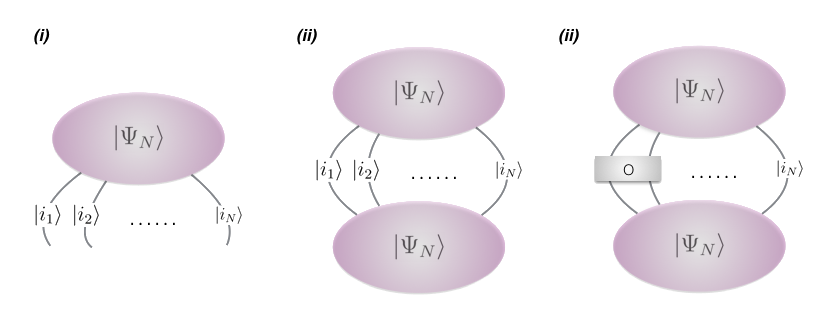
\includegraphics[width=0.75\textwidth]{figures/fig225.png}
	\caption[Represent wave-function of quntum states of TN]{(i) The wave-function, $\Ket{\Psi_N}$ (ii) The norm of $\Ket{\Psi_N}$, $\Braket{\Psi_N|\Psi_N}$ (iii) Expectation value of observable $O$, $\Bra{\Psi_N}O\Ket{\Psi_N}$}
	\label{fig225}
\end{figure}

\section{Matrix product state}
\label{MPS}

%The wave-function composed by pure states can be decompose into many unit cells by \textit{sigular value decomopostion} and \textit{Schmidt decomposition}. 
A pure state wave function can be written as a sum of product of bipartite wave functions. We begin from splitting the wave-function $\Ket{\Psi_N}$ [Fig.~\ref{fig225}(a)] between $n$ and $n+1$ sites with Schmidt decomposition, 
\begin{align}
	\label{schmitwave}
	\Ket{\Psi_{N}} = \sum_{\alpha_n} \lambda_{\alpha_n} \Ket{\psi_{\alpha_n}^{[1\dots n]}} \Ket{\psi_{\alpha_n}^{[n+1\dots N]}}
\end{align}
where $\lambda_{\alpha_n} > 0$ and $\sum\limits_{\alpha_n}{\lambda_{\alpha_n}^2 = 1}$. To obtain the one site wave function $\Ket{\psi_{\alpha_n}^{[n+1]}}$, we perform Schmidt decomposition on $\Ket{\psi_{\alpha_n}^{[n+1\dots N]}}$ between the $n+1$ and $n+2$ sites,
\begin{align}
	\Ket{\psi_{\alpha_n}^{[n+1\dots N]}} = \sum_{\alpha_{n+1}} \lambda_{\alpha_{n+1}} \Ket{\psi_{\alpha_{n+1}}^{[n+1]}} \Ket{\psi_{\alpha_{n+2}}^{[n+2\dots N]}}
\end{align}
then span $\Ket{\psi_{\alpha_{n+1}}^{[n+1]}}$ by the spin basis $i_{n+1}$,
\begin{align}
	\Ket{\psi_{\alpha_{n+1}}^{[n+1]}} = \sum_{i_{n+1}}{\Gamma^{[n+1] i_{n+1}}_{\alpha_n \alpha_{n+1}} \Ket{i_{n+1}}}
\end{align}
and the Eq. \ref{schmitwave} can be rewritten as
\begin{align}
	\Ket{\Psi_{N}} = \sum_{\alpha_n,\alpha_{n+1}}\sum_{i_{n+1}}{\lambda_{\alpha_n} \Gamma^{[n+1] i_{n+1}}_{\alpha_n \alpha_{n+1}} \lambda_{\alpha_{n+1}l} \Ket{\psi_{\alpha_n}^{[1\dots n]}} \Ket{i_{n+1}} \Ket{\psi_{\alpha_{n+2}}^{[n+2\dots N]}} }
\end{align}
In the end, we can repeat the same process site-by-site in the entire system and obtain the MPS structure,
\begin{align}
	\Ket{\Psi_N} = \sum_{\alpha_1,\dots ,\alpha_N}\sum_{i_1,\dots ,i_N}{ \Gamma^{[1] i_{1}}_{\alpha_1} \lambda_{\alpha_1} \Gamma^{[2] i_{2}}_{\alpha_1 \alpha_{2}} \lambda_{\alpha_2} \dots  \lambda_{\alpha_{N-2}} \Gamma^{[N-1] i_{N-1}}_{\alpha_{N-2} \alpha_{N-1}} \lambda_{\alpha_{N-1}} \Gamma^{[N] i_{N}}_{\alpha_{N}} \Ket{i_1 i_2 \dots i_N}}
\end{align}
and the tensor network representation is shown as Fig.~\ref{fig311}. So far the decomposition is exact, and an approximate MPS can be constructed by cutting of the dimensions of $\lambda$

Now we try to expand it to an infinite chain \cite{PhysRevLett.98.070201}. Due to the translational invariance, the wave function $\Ket{\Psi_{N=\infty}}$ can be represented as $n$-site translational symmetric states, which means that $\Gamma^{[i]}$ and $\lambda^{[i_{i}]}$ are independent of $\Gamma^{[i+n]}$ and $\lambda^{[i+n]}$. For instance, when $n=2$, the wave-function of an infinite chain can be recognized as a composite of two different matrix product states $\lambda^{[A]}\Gamma^{[A]}$ (red nodes) and $\lambda^{[B]}\Gamma^{[B]}$ (purple nodes), as shown in Fig.\ref{fig312}. Therefore, the requirement of the coefficients is reduced from $d^N$ to $NdD^2$, where $D$ is bond dimension between each matrix product states and we also call it virtual bond dimension. 
%%%%%%%%%%%%%%%%%%%
This can be extended to 2D 
in the following chapters, we will use MPS and PEPS as our variational wave function to study quantum many-body systems.
%%%%%%%%%%%%%%%%%%%

\begin{figure}[hb]
	\centering
	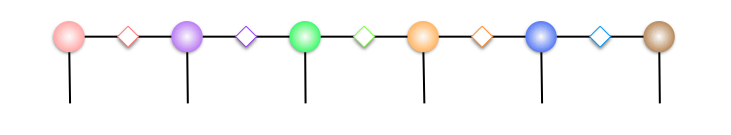
\includegraphics[width=0.90\textwidth]{figures/fig3111.png}
	\caption[The tensor network representation of matrix product states]{The tensor network representation of a matrix product state.}
	\label{fig311}
\end{figure}

\begin{figure}[hb]
	\centering
	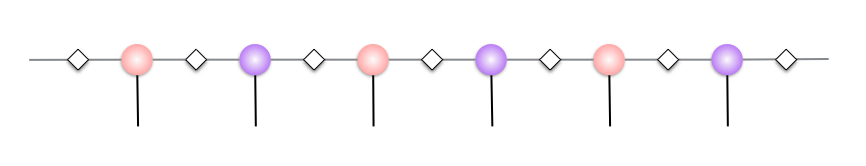
\includegraphics[width=0.90\textwidth]{figures/fig311.png}
	\caption[The tensor network representation of infinite matrix product states]{The tensor network representation of an infinite matrix product state.}
	\label{fig312}
\end{figure}
